% Options for packages loaded elsewhere
\PassOptionsToPackage{unicode}{hyperref}
\PassOptionsToPackage{hyphens}{url}
\PassOptionsToPackage{dvipsnames,svgnames,x11names}{xcolor}
%
\documentclass[
  letterpaper,
  DIV=11,
  numbers=noendperiod]{scrartcl}

\usepackage{amsmath,amssymb}
\usepackage{iftex}
\ifPDFTeX
  \usepackage[T1]{fontenc}
  \usepackage[utf8]{inputenc}
  \usepackage{textcomp} % provide euro and other symbols
\else % if luatex or xetex
  \usepackage{unicode-math}
  \defaultfontfeatures{Scale=MatchLowercase}
  \defaultfontfeatures[\rmfamily]{Ligatures=TeX,Scale=1}
\fi
\usepackage{lmodern}
\ifPDFTeX\else  
    % xetex/luatex font selection
\fi
% Use upquote if available, for straight quotes in verbatim environments
\IfFileExists{upquote.sty}{\usepackage{upquote}}{}
\IfFileExists{microtype.sty}{% use microtype if available
  \usepackage[]{microtype}
  \UseMicrotypeSet[protrusion]{basicmath} % disable protrusion for tt fonts
}{}
\makeatletter
\@ifundefined{KOMAClassName}{% if non-KOMA class
  \IfFileExists{parskip.sty}{%
    \usepackage{parskip}
  }{% else
    \setlength{\parindent}{0pt}
    \setlength{\parskip}{6pt plus 2pt minus 1pt}}
}{% if KOMA class
  \KOMAoptions{parskip=half}}
\makeatother
\usepackage{xcolor}
\setlength{\emergencystretch}{3em} % prevent overfull lines
\setcounter{secnumdepth}{-\maxdimen} % remove section numbering
% Make \paragraph and \subparagraph free-standing
\makeatletter
\ifx\paragraph\undefined\else
  \let\oldparagraph\paragraph
  \renewcommand{\paragraph}{
    \@ifstar
      \xxxParagraphStar
      \xxxParagraphNoStar
  }
  \newcommand{\xxxParagraphStar}[1]{\oldparagraph*{#1}\mbox{}}
  \newcommand{\xxxParagraphNoStar}[1]{\oldparagraph{#1}\mbox{}}
\fi
\ifx\subparagraph\undefined\else
  \let\oldsubparagraph\subparagraph
  \renewcommand{\subparagraph}{
    \@ifstar
      \xxxSubParagraphStar
      \xxxSubParagraphNoStar
  }
  \newcommand{\xxxSubParagraphStar}[1]{\oldsubparagraph*{#1}\mbox{}}
  \newcommand{\xxxSubParagraphNoStar}[1]{\oldsubparagraph{#1}\mbox{}}
\fi
\makeatother

\usepackage{color}
\usepackage{fancyvrb}
\newcommand{\VerbBar}{|}
\newcommand{\VERB}{\Verb[commandchars=\\\{\}]}
\DefineVerbatimEnvironment{Highlighting}{Verbatim}{commandchars=\\\{\}}
% Add ',fontsize=\small' for more characters per line
\usepackage{framed}
\definecolor{shadecolor}{RGB}{241,243,245}
\newenvironment{Shaded}{\begin{snugshade}}{\end{snugshade}}
\newcommand{\AlertTok}[1]{\textcolor[rgb]{0.68,0.00,0.00}{#1}}
\newcommand{\AnnotationTok}[1]{\textcolor[rgb]{0.37,0.37,0.37}{#1}}
\newcommand{\AttributeTok}[1]{\textcolor[rgb]{0.40,0.45,0.13}{#1}}
\newcommand{\BaseNTok}[1]{\textcolor[rgb]{0.68,0.00,0.00}{#1}}
\newcommand{\BuiltInTok}[1]{\textcolor[rgb]{0.00,0.23,0.31}{#1}}
\newcommand{\CharTok}[1]{\textcolor[rgb]{0.13,0.47,0.30}{#1}}
\newcommand{\CommentTok}[1]{\textcolor[rgb]{0.37,0.37,0.37}{#1}}
\newcommand{\CommentVarTok}[1]{\textcolor[rgb]{0.37,0.37,0.37}{\textit{#1}}}
\newcommand{\ConstantTok}[1]{\textcolor[rgb]{0.56,0.35,0.01}{#1}}
\newcommand{\ControlFlowTok}[1]{\textcolor[rgb]{0.00,0.23,0.31}{\textbf{#1}}}
\newcommand{\DataTypeTok}[1]{\textcolor[rgb]{0.68,0.00,0.00}{#1}}
\newcommand{\DecValTok}[1]{\textcolor[rgb]{0.68,0.00,0.00}{#1}}
\newcommand{\DocumentationTok}[1]{\textcolor[rgb]{0.37,0.37,0.37}{\textit{#1}}}
\newcommand{\ErrorTok}[1]{\textcolor[rgb]{0.68,0.00,0.00}{#1}}
\newcommand{\ExtensionTok}[1]{\textcolor[rgb]{0.00,0.23,0.31}{#1}}
\newcommand{\FloatTok}[1]{\textcolor[rgb]{0.68,0.00,0.00}{#1}}
\newcommand{\FunctionTok}[1]{\textcolor[rgb]{0.28,0.35,0.67}{#1}}
\newcommand{\ImportTok}[1]{\textcolor[rgb]{0.00,0.46,0.62}{#1}}
\newcommand{\InformationTok}[1]{\textcolor[rgb]{0.37,0.37,0.37}{#1}}
\newcommand{\KeywordTok}[1]{\textcolor[rgb]{0.00,0.23,0.31}{\textbf{#1}}}
\newcommand{\NormalTok}[1]{\textcolor[rgb]{0.00,0.23,0.31}{#1}}
\newcommand{\OperatorTok}[1]{\textcolor[rgb]{0.37,0.37,0.37}{#1}}
\newcommand{\OtherTok}[1]{\textcolor[rgb]{0.00,0.23,0.31}{#1}}
\newcommand{\PreprocessorTok}[1]{\textcolor[rgb]{0.68,0.00,0.00}{#1}}
\newcommand{\RegionMarkerTok}[1]{\textcolor[rgb]{0.00,0.23,0.31}{#1}}
\newcommand{\SpecialCharTok}[1]{\textcolor[rgb]{0.37,0.37,0.37}{#1}}
\newcommand{\SpecialStringTok}[1]{\textcolor[rgb]{0.13,0.47,0.30}{#1}}
\newcommand{\StringTok}[1]{\textcolor[rgb]{0.13,0.47,0.30}{#1}}
\newcommand{\VariableTok}[1]{\textcolor[rgb]{0.07,0.07,0.07}{#1}}
\newcommand{\VerbatimStringTok}[1]{\textcolor[rgb]{0.13,0.47,0.30}{#1}}
\newcommand{\WarningTok}[1]{\textcolor[rgb]{0.37,0.37,0.37}{\textit{#1}}}

\providecommand{\tightlist}{%
  \setlength{\itemsep}{0pt}\setlength{\parskip}{0pt}}\usepackage{longtable,booktabs,array}
\usepackage{calc} % for calculating minipage widths
% Correct order of tables after \paragraph or \subparagraph
\usepackage{etoolbox}
\makeatletter
\patchcmd\longtable{\par}{\if@noskipsec\mbox{}\fi\par}{}{}
\makeatother
% Allow footnotes in longtable head/foot
\IfFileExists{footnotehyper.sty}{\usepackage{footnotehyper}}{\usepackage{footnote}}
\makesavenoteenv{longtable}
\usepackage{graphicx}
\makeatletter
\newsavebox\pandoc@box
\newcommand*\pandocbounded[1]{% scales image to fit in text height/width
  \sbox\pandoc@box{#1}%
  \Gscale@div\@tempa{\textheight}{\dimexpr\ht\pandoc@box+\dp\pandoc@box\relax}%
  \Gscale@div\@tempb{\linewidth}{\wd\pandoc@box}%
  \ifdim\@tempb\p@<\@tempa\p@\let\@tempa\@tempb\fi% select the smaller of both
  \ifdim\@tempa\p@<\p@\scalebox{\@tempa}{\usebox\pandoc@box}%
  \else\usebox{\pandoc@box}%
  \fi%
}
% Set default figure placement to htbp
\def\fps@figure{htbp}
\makeatother

\KOMAoption{captions}{tableheading}
\makeatletter
\@ifpackageloaded{caption}{}{\usepackage{caption}}
\AtBeginDocument{%
\ifdefined\contentsname
  \renewcommand*\contentsname{Table of contents}
\else
  \newcommand\contentsname{Table of contents}
\fi
\ifdefined\listfigurename
  \renewcommand*\listfigurename{List of Figures}
\else
  \newcommand\listfigurename{List of Figures}
\fi
\ifdefined\listtablename
  \renewcommand*\listtablename{List of Tables}
\else
  \newcommand\listtablename{List of Tables}
\fi
\ifdefined\figurename
  \renewcommand*\figurename{Figure}
\else
  \newcommand\figurename{Figure}
\fi
\ifdefined\tablename
  \renewcommand*\tablename{Table}
\else
  \newcommand\tablename{Table}
\fi
}
\@ifpackageloaded{float}{}{\usepackage{float}}
\floatstyle{ruled}
\@ifundefined{c@chapter}{\newfloat{codelisting}{h}{lop}}{\newfloat{codelisting}{h}{lop}[chapter]}
\floatname{codelisting}{Listing}
\newcommand*\listoflistings{\listof{codelisting}{List of Listings}}
\makeatother
\makeatletter
\makeatother
\makeatletter
\@ifpackageloaded{caption}{}{\usepackage{caption}}
\@ifpackageloaded{subcaption}{}{\usepackage{subcaption}}
\makeatother

\usepackage{bookmark}

\IfFileExists{xurl.sty}{\usepackage{xurl}}{} % add URL line breaks if available
\urlstyle{same} % disable monospaced font for URLs
\hypersetup{
  pdftitle={Premliminary Analysis},
  pdfauthor={Ken Kabeya \& Aneesh Koppolu},
  colorlinks=true,
  linkcolor={blue},
  filecolor={Maroon},
  citecolor={Blue},
  urlcolor={Blue},
  pdfcreator={LaTeX via pandoc}}


\title{Premliminary Analysis}
\author{Ken Kabeya \& Aneesh Koppolu}
\date{}

\begin{document}
\maketitle

\renewcommand*\contentsname{Table of contents}
{
\hypersetup{linkcolor=}
\setcounter{tocdepth}{3}
\tableofcontents
}

Preliminary Analysis

\begin{center}\rule{0.5\linewidth}{0.5pt}\end{center}

\subsection{\texorpdfstring{\textbf{Introduction}}{Introduction}}\label{introduction}

The Rugby World Cup (RWC) is the most prestigious tournament in men's
international rugby, held every four years and featuring the
top-performing nations from around the globe. Since its inception in
1987, all winning teams have come from the group of tier-one rugby
nations---those with well-established professional structures and a
history of competitive success. The World Cup's high stakes, unique
pressure, and knockout format often produce different outcomes from
regular international fixtures, yet the path to RWC success may still be
written in a team's performance leading up to the tournament.

This project seeks to bridge our understanding of regular international
performance with World Cup outcomes through a predictive modeling lens.
Our guiding research question is:\\
\textgreater{} \textbf{Can regular fixture performance since 1999
reliably predict World Cup success for tier-one rugby nations?}

We expect that teams with consistently high win rates, dominant scoring
margins, and strong rankings (e.g., Elo ratings) leading into a World
Cup are more likely to progress further or win the tournament. Based on
our model, and consistent with historical trends, we predict that
\textbf{South Africa (RSA)}, \textbf{Ireland (IRE)}, or \textbf{New
Zealand (NZ)} are the most likely candidates to win the 2027 Rugby World
Cup.

\begin{center}\rule{0.5\linewidth}{0.5pt}\end{center}

\subsection{\texorpdfstring{\textbf{Data}}{Data}}\label{data}

\subsubsection{\texorpdfstring{\textbf{Data Source and
Collection}}{Data Source and Collection}}\label{data-source-and-collection}

The data for this project was sourced from an international rugby match
dataset containing results from test matches played by men's national
teams. The dataset includes \textbf{2,783 matches}, of which
\textbf{1,230} were retained after filtering for: - Matches played
\textbf{between 1999 and 2024}, inclusive - \textbf{Tier-one teams} only
- Complete match records (with no missing scores or team names)

\subsubsection{\texorpdfstring{\textbf{Cases and
Variables}}{Cases and Variables}}\label{cases-and-variables}

Each row in the dataset represents a single international rugby match
and includes variables such as: - \texttt{date}: Match date -
\texttt{home\_team}, \texttt{away\_team}: Competing teams -
\texttt{home\_score}, \texttt{away\_score}: Points scored by each team -
\texttt{competition}: Type of match (e.g., World Cup, Six Nations, etc.)
- \texttt{neutral}: Boolean indicator for neutral venue -
\texttt{world\_cup}: Boolean indicator for whether the match is a World
Cup fixture

\subsubsection{\texorpdfstring{\textbf{Data Wrangling and Feature
Engineering}}{Data Wrangling and Feature Engineering}}\label{data-wrangling-and-feature-engineering}

To support our analysis, we created several new variables and tidied the
dataset: - Extracted \texttt{year} from the match date for time-series
analysis - Created binary indicators: \texttt{homeWin} and
\texttt{awayWin} - Calculated \texttt{count} to aid in aggregating match
totals - Grouped matches by team to calculate: - \textbf{Home and away
win percentages} - \textbf{Average points scored and conceded (home and
away)} - \textbf{World Cup vs.~regular fixture performance} - Developed
year-by-year win percentage timelines for each team

\subsubsection{\texorpdfstring{\textbf{Variables for
Modeling}}{Variables for Modeling}}\label{variables-for-modeling}

We plan to include the following variables in our predictive models: -
\textbf{Win Percentage (last 2 years before RWC)}: Measures recent
performance - \textbf{Average Point Differential}: Offensive and
defensive strength indicator - \textbf{Elo Rating} (if included or
computed): Captures opponent-adjusted team strength - \textbf{Tournament
Flag}: Helps compare regular matches to World Cup fixtures -
\textbf{Home/Away Advantage}: Quantified through win rates and score
differentials

These variables were chosen for their interpretability and demonstrated
relevance in differentiating strong and weak tournament performers.

\begin{center}\rule{0.5\linewidth}{0.5pt}\end{center}

\subsection{\texorpdfstring{\textbf{Methodology}}{Methodology}}\label{methodology}

\subsubsection{\texorpdfstring{\textbf{Research
Question}}{Research Question}}\label{research-question}

Our goal is to explore whether consistent performance in international
fixtures since 1999 can predict a team's success at the Rugby World Cup
(RWC). We focus on tier-one nations, and based on trends in both regular
and tournament data, we aim to forecast the winner of the 2027 RWC. Our
preliminary model predicts that \textbf{South Africa, Ireland, or New
Zealand} are the most likely champions.

\begin{center}\rule{0.5\linewidth}{0.5pt}\end{center}

\subsubsection{\texorpdfstring{\textbf{Data Overview and
Cleaning}}{Data Overview and Cleaning}}\label{data-overview-and-cleaning}

We used a dataset containing \textbf{2,783 international matches}, which
was filtered to: - \textbf{Matches after 1998}, yielding \textbf{1,230
matches}. - \textbf{Tier-one teams only}, excluding matches with
insufficient data or unclear team tier.

Cleaning Steps: - Extracted \textbf{year} from match dates for temporal
analysis. - Created binary flags for \textbf{homeWin} and
\textbf{awayWin}. - Dropped rows with missing values. - Created a
\textbf{``count''} variable to aggregate matches played per team.

\begin{center}\rule{0.5\linewidth}{0.5pt}\end{center}

\subsubsection{\texorpdfstring{\textbf{Feature Engineering and
Wrangling}}{Feature Engineering and Wrangling}}\label{feature-engineering-and-wrangling}

We created several new variables from existing match data: -
\textbf{Home/Away Win Percentages}: Calculated by aggregating match
results per team. - \textbf{Average Points Scored and Conceded}: For
both World Cup and non-World Cup matches. - \textbf{World Cup Match
Flag}: To compare regular vs.~tournament performance. - \textbf{Yearly
Win Percentage}: A normalized view of performance over time per team.

\begin{quote}
Code implementation used pandas and NumPy, with seaborn and matplotlib
for plotting.
\end{quote}

\begin{center}\rule{0.5\linewidth}{0.5pt}\end{center}

\subsubsection{\texorpdfstring{\textbf{Exclusions}}{Exclusions}}\label{exclusions}

We excluded: - All matches involving \textbf{non-tier-one nations}. -
Matches with \textbf{missing scores} or unclear venues. -
Non-competitive matches that could skew performance metrics (e.g.,
experimental squads).

\begin{center}\rule{0.5\linewidth}{0.5pt}\end{center}

\subsubsection{\texorpdfstring{\textbf{Summary
Statistics}}{Summary Statistics}}\label{summary-statistics}

\begin{longtable}[]{@{}lllll@{}}
\toprule\noalign{}
Variable & Mean & Std Dev & Min & Max \\
\midrule\noalign{}
\endhead
\bottomrule\noalign{}
\endlastfoot
Home Score & 25.07 & 13.15 & 0 & 101 \\
Away Score & 20.78 & 11.38 & 0 & 68 \\
Home Win Rate & 59.6\% & --- & 0 & 1 \\
Away Win Rate & 38.4\% & --- & 0 & 1 \\
Year & 2011.5 & 7.2 & 1999 & 2024 \\
\end{longtable}

\textbf{Observation}:\\
On average, the \textbf{home team outperforms the away team by
\textasciitilde4.3 points}. The home win rate is significantly higher
across all teams.

\begin{longtable}[]{@{}
  >{\raggedright\arraybackslash}p{(\linewidth - 0\tabcolsep) * \real{1.0000}}@{}}
\toprule\noalign{}
\endhead
\bottomrule\noalign{}
\endlastfoot
\#\#\# \textbf{Key Visualizations} \\
\textbf{1. Home and Away Win Rates by Team}  \\
::: \{.cell execution\_count=1\} \\
::: \{.cell-output .cell-output-display execution\_count=1\} \\
::: \{.cell execution\_count=2\} ``` \{.python .cell-code\} \#only
keeping data after 1999 \#will create a year col and then trim the
data \\
rugbyDF{[}`year'{]} = rugbyDF{[}`date'{]}.str{[}0:4{]}.astype(int)
rugbyDF = rugbyDF{[}rugbyDF.year \textgreater{} 1998{]}
rugbyDF.dropna(inplace = True) rugbyDF.shape \#new shape of dataframe:
(1230,12) ``` \\
::: \{.cell-output .cell-output-display execution\_count=2\} \\
::: \{.cell execution\_count=3\} ``` \{.python .cell-code\} \#creating
variable to track if home or away team won \#created weights for win,
draw, and loss rugbyDF{[}``homeWin''{]} =
np.where(rugbyDF{[}``home\_score''{]} \textgreater{}
rugbyDF{[}``away\_score''{]}, 1,0) rugbyDF{[}``awayWin''{]} =
np.where(rugbyDF{[}``home\_score''{]} \textless{}
rugbyDF{[}``away\_score''{]}, 1,0) \\
\#creating a count var to help with num of games played later on
rugbyDF{[}``count''{]} = 1 ``` ::: \\
::: \{.cell execution\_count=4\} ``` \{.python .cell-code\} for cols in
rugbyDF.columns: print(cols + ``:'' + (str)(rugbyDF{[}cols{]}.dtype)) \\
\#Since there are 2 numerical cols, i can get summary statistics on them
\#year variable will not be taken into account for summary statistics
rugbyDF.describe() ``` \\
::: \{.cell-output .cell-output-stdout\} \\
::: \{.cell-output .cell-output-display execution\_count=4\} \\
```\{=html\} \\
.dataframe tbody tr th \{ vertical-align: top; \} \\
.dataframe thead th \{ text-align: right; \} \\
::: ::: \\
We can observe that the mean points scored by the home team was
approximately 4.2 higher than the away team. All major quadrants have
higher points for home\_score than away\_score, and the std is also
greater. \\
We also notice that the home team won \textasciitilde59.6\%* of the
games contested. \\
*This does not account for games that take place in neutral venues. \\
::: \{.cell execution\_count=5\} ``` \{.python .cell-code\} \#create
diff df by teams, then find the summary statistics for those teams.
unq\_hteams = rugbyDF{[}`home\_team'{]}.unique() unq\_ateams =
rugbyDF{[}`away\_team'{]}.unique() unq\_teams = np.unique((unq\_hteams,
unq\_ateams)) unq\_teams \\
\#shortens the df to only include awayteam, awaywin or hometeam, homewin
rugbyDFH = rugbyDF{[}{[}``home\_team'',``homeWin'',``count''{]}{]}
rugbyDFA = rugbyDF{[}{[}``away\_team'',``awayWin'',``count''{]}{]} \\
\#groups the data by team groupedH =
rugbyDFH.groupby(`home\_team').sum() groupedA =
rugbyDFA.groupby(`away\_team').sum() \\
\#renames the axis to the same thing groupedA =
groupedA.rename\_axis(`team') groupedH =
groupedH.rename\_axis(`team') \\
\#find team win percentage by away and home
groupedH{[}``home\_win\%''{]} =
groupedH{[}``homeWin''{]}/groupedH{[}``count''{]} \emph{100
groupedA{[}``away\_win\%''{]} =
groupedA{[}``awayWin''{]}/groupedA{[}``count''{]} }100 \\
\#renames count so that they dont clash when merging groupedH =
groupedH.rename(columns=\{`count': `count\_home'\}) groupedA =
groupedA.rename(columns=\{`count': `count\_away'\}) \\
\#merge the data frames teams\_wins = pd.merge(groupedH, groupedA,
on=`team', how=`inner') teams\_wins ``` \\
::: \{.cell-output .cell-output-display execution\_count=5\} \\
```\{=html\} \\
.dataframe tbody tr th \{ vertical-align: top; \} \\
.dataframe thead th \{ text-align: right; \} \\
::: ::: \\
This data frame represents the team wise performance breakdown from
1999-2024. \\
::: \{.cell execution\_count=6\} ``` \{.python .cell-code\} fig, ax =
plt.subplots() \\
y = np.arange(len(unq\_teams)) \# Team positions width = 0.37 \# Bar
width \\
plt.barh(y - width/2, teams\_wins{[}``home\_win\%''{]}, width,
label=`Home Win \%') plt.barh(y + width/2,
teams\_wins{[}``away\_win\%''{]}, width, label=`Away Win \%')
plt.yticks(y, unq\_teams) \\
\# Add labels and title plt.ylabel(`Teams') plt.xlabel(`Home Win\% and
Away Win\%') plt.title(`Home and Away Win Percentage By Team') \\
plt.legend() fig.tight\_layout() plt.show() plt.close() ``` \\
::: \{.cell-output .cell-output-display\}
\pandocbounded{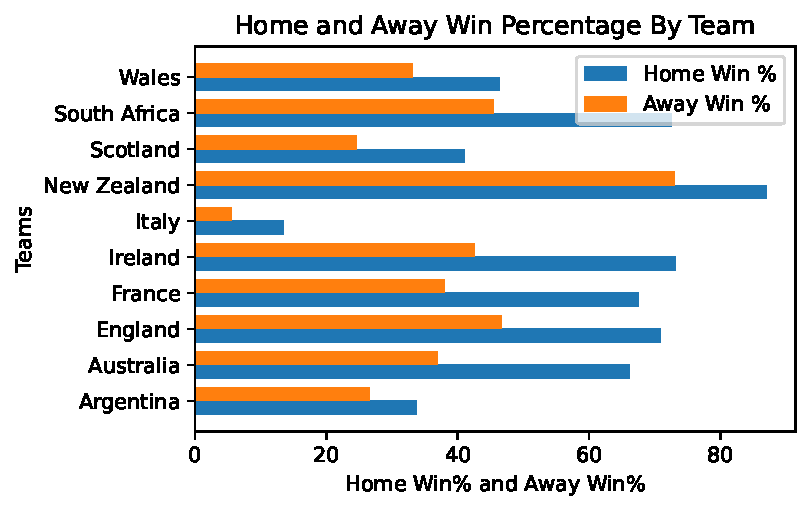
\includegraphics[keepaspectratio]{Preliminary Analysis_files/figure-pdf/cell-7-output-1.pdf}}
::: ::: \\
- New Zealand dominates both at home and away. - All teams perform
\textbf{better at home}, confirming home advantage. - Italy
underperforms consistently. \\
\textbf{2. Average Points Scored vs.~Conceded} - Teams like \textbf{New
Zealand} and \textbf{South Africa} show high scores with low concession.
- \textbf{Italy} and \textbf{Scotland} concede more than they score,
especially in away games. \\
::: \{.cell execution\_count=7\} ``` \{.python .cell-code\} \#a function
to create a scoring dataset def createscoringdataset(rugbyDF): \\
\#shortens the df to only include awayteam, awaywin or hometeam, homewin
rugbyDFH\_score =
rugbyDF{[}{[}``home\_team'',``home\_score'',``away\_score'',``count''{]}{]}
rugbyDFA\_score =
rugbyDF{[}{[}``away\_team'',``away\_score'',``home\_score'',``count''{]}{]} \\
\#renaming away\_score and home\_score to home\_conceded and
away\_conceded rugbyDFH\_score =
rugbyDFH\_score.rename(columns=\{`away\_score': `home\_conceded'\})
rugbyDFA\_score = rugbyDFA\_score.rename(columns=\{`home\_score':
`away\_conceded'\}) \\
\#groups the data by team groupedH\_score =
rugbyDFH\_score.groupby(`home\_team').sum() groupedA\_score =
rugbyDFA\_score.groupby(`away\_team').sum() \\
\#renames the axis to the same thing groupedH\_score =
groupedH\_score.rename\_axis(`team') groupedA\_score =
groupedA\_score.rename\_axis(`team') \\
\#merge the data frames teams\_score = pd.merge(groupedH\_score,
groupedA\_score, on=`team', how=`inner') \\
\#rename count\_x and count\_y to home\_played and away\_played
teams\_score = teams\_score.rename(columns=\{`count\_x': `home\_played',
`count\_y': `away\_played'\}) \\
\#find team win percentage by away and home
teams\_score{[}``home\_score\_avg''{]} =
teams\_score{[}``home\_score''{]}/teams\_score{[}``home\_played''{]}
teams\_score{[}``away\_score\_avg''{]} =
teams\_score{[}``away\_score''{]}/teams\_score{[}``away\_played''{]} \\
teams\_score{[}``home\_conceded\_avg''{]} =
teams\_score{[}``home\_conceded''{]}/teams\_score{[}``home\_played''{]}
teams\_score{[}``away\_conceded\_avg''{]} =
teams\_score{[}``away\_conceded''{]}/teams\_score{[}``away\_played''{]}
return teams\_score \\
teams\_score = createscoringdataset(rugbyDF) ``` ::: \\
::: \{.cell execution\_count=8\} ``` \{.python .cell-code\} \# Create a
2x2 grid of subplots fig, axs = plt.subplots(2, 2) \# 2 rows, 2
columns \\
\# Add main title fig.suptitle(``Teamwise Home vs Away Performance'',
fontsize=16, y=1.02, \# Adjust vertical position (1.0 = top of plot)
fontweight=`bold') \\
\# Plot 1: Home Win \% axs{[}0, 0{]}.barh(unq\_teams,
teams\_wins{[}``home\_win\%''{]}, color=`blue') axs{[}0,
0{]}.set\_title(`Home Win Percentage') axs{[}0, 0{]}.set\_xlabel(`Win
\%') \\
\# Plot 2: Away Win \% axs{[}0, 1{]}.barh(unq\_teams,
teams\_wins{[}``away\_win\%''{]}, color=`orange') axs{[}0,
1{]}.set\_title(`Away Win Percentage') axs{[}0, 1{]}.set\_xlabel(`Win
\%') \\
\# Plot 3: Home vs Away Comparison (side-by-side) y =
range(len(unq\_teams)) width = 0.35 axs{[}1, 0{]}.barh({[}y - width/2
for y in y{]}, teams\_wins{[}``home\_win\%''{]}, width, label=`Home',
color=`blue') axs{[}1, 0{]}.barh({[}y + width/2 for y in y{]},
teams\_wins{[}``away\_win\%''{]}, width, label=`Away', color=`orange')
axs{[}1, 0{]}.set\_title(`Home vs Away Comparison') axs{[}1,
0{]}.set\_xlabel(`Win \%') axs{[}1, 0{]}.set\_yticks(y) axs{[}1,
0{]}.set\_yticklabels(unq\_teams) axs{[}1, 0{]}.legend() \\
\# Plot 4: Difference (Home - Away) axs{[}1, 1{]}.barh(unq\_teams,
teams\_wins{[}``home\_win\%''{]} - teams\_wins{[}``away\_win\%''{]},
color=`green') axs{[}1, 1{]}.set\_title(`Home Advantage (Home - Away)')
axs{[}1, 1{]}.set\_xlabel(`Win \% Difference') \\
plt.tight\_layout(rect={[}0.00, 0.0, 1, 1{]}) \# Adjusts spacing between
subplots plt.subplots\_adjust(wspace=0.7, hspace=0.6) plt.show()
plt.close() ``` \\
::: \{.cell-output .cell-output-display\}
\pandocbounded{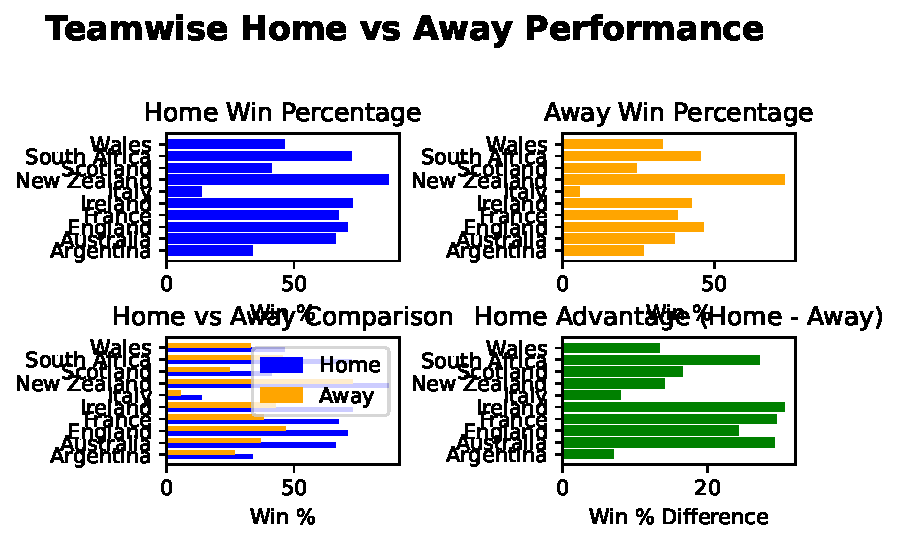
\includegraphics[keepaspectratio]{Preliminary Analysis_files/figure-pdf/cell-9-output-1.pdf}}
::: ::: \\
\textbf{3. World Cup vs.~Regular Match Comparison} - \textbf{Ireland and
South Africa} maintain strong performance in both contexts. - Some teams
\textbf{drop significantly in performance during World Cups}, revealing
tournament pressure or lack of depth. \\
::: \{.cell execution\_count=9\} ``` \{.python .cell-code\} \#creates
world cup scoring df \\
worldCupDF = rugbyDF{[}rugbyDF.world\_cup == True{]} nonWorldCup =
rugbyDF{[}rugbyDF.world\_cup == False{]} wc\_scoring =
createscoringdataset(worldCupDF) non\_wc\_scoring =
createscoringdataset(nonWorldCup) ``` ::: \\
::: \{.cell execution\_count=10\} ``` \{.python .cell-code\} \# Create a
2x2 grid of subplots fig, axs = plt.subplots(2, 2) \# 2 rows, 2
columns \\
\# Add main title fig.suptitle(``World Cup vs Non World Cup Offense and
Defense'', fontsize=16, y=1.02, \# Adjust vertical position (1.0 = top
of plot) fontweight=`bold') \\
\# Plot 1: World Cup vs Non World Cup home-score-avg y =
range(len(unq\_teams)) width = 0.35 axs{[}0, 0{]}.barh({[}y - width/2
for y in y{]}, wc\_scoring{[}`home\_score\_avg'{]}, width, label=`World
Cup', color=`\#D4AF37') axs{[}0, 0{]}.barh({[}y + width/2 for y in y{]},
non\_wc\_scoring{[}`home\_score\_avg'{]}, width, label=`Non World Cup',
color=`\#A6A6A6') axs{[}0, 0{]}.set\_title(`Home Points') axs{[}0,
0{]}.set\_xlabel(`Avg Points') axs{[}0, 0{]}.set\_yticks(y) axs{[}0,
0{]}.set\_yticklabels(unq\_teams) \\
\# Plot 2: World Cup vs Non World Cup away-score-avg axs{[}1,
0{]}.barh({[}y - width/2 for y in y{]},
wc\_scoring{[}`away\_score\_avg'{]}, width, label=`World Cup',
color=`\#D4AF37') axs{[}1, 0{]}.barh({[}y + width/2 for y in y{]},
non\_wc\_scoring{[}`away\_score\_avg'{]}, width, label=`Non World Cup',
color=`\#A6A6A6') axs{[}1, 0{]}.set\_title(`Away Points') axs{[}1,
0{]}.set\_xlabel(`Avg Points') axs{[}1, 0{]}.set\_yticks(y) axs{[}1,
0{]}.set\_yticklabels(unq\_teams) \\
\# Plot 3: World Cup vs Non World Cup home-conceded-avg axs{[}0,
1{]}.barh({[}y - width/2 for y in y{]},
wc\_scoring{[}`home\_conceded\_avg'{]}, width, label=`World Cup',
color=`\#D4AF37') axs{[}0, 1{]}.barh({[}y + width/2 for y in y{]},
non\_wc\_scoring{[}`home\_conceded\_avg'{]}, width, label=`Non World
Cup', color=`\#A6A6A6') axs{[}0, 1{]}.set\_title(`Home Conceded')
axs{[}0, 1{]}.set\_xlabel(`Avg Points') axs{[}0, 1{]}.set\_yticks(y)
axs{[}0, 1{]}.set\_yticklabels(unq\_teams) \\
\# Plot 4: World Cup vs Non World Cup away-conceded-avg axs{[}1,
1{]}.barh({[}y - width/2 for y in y{]},
wc\_scoring{[}`away\_conceded\_avg'{]}, width, label=`World Cup',
color=`\#D4AF37') axs{[}1, 1{]}.barh({[}y + width/2 for y in y{]},
non\_wc\_scoring{[}`away\_conceded\_avg'{]}, width, label=`Non World
Cup', color=`\#A6A6A6') axs{[}1, 1{]}.set\_title(`Away Conceded')
axs{[}1, 1{]}.set\_xlabel(`Avg Points') axs{[}1, 1{]}.set\_yticks(y)
axs{[}1, 1{]}.set\_yticklabels(unq\_teams) \\
\# Create invisible artist in center
fig.patches.extend({[}plt.Rectangle((0.5, 0.5), 0.01, 0.01, alpha=0,
zorder=100, transform=fig.transFigure){]}) \\
\# Create unified legend legend\_elements = {[} plt.Rectangle((0,0), 1,
1, fc=`\#D4AF37', ec=`\#B8860B', lw=1, label=`WC'), plt.Rectangle((0,0),
1, 1, fc=`\#A6A6A6', ec=`\#808080', lw=1, label=`Non WC'){]} \\
\# Place legend in absolute center legend =
fig.legend(handles=legend\_elements, loc=`center',
bbox\_to\_anchor=(0.60, 0.49), \# Dead center
bbox\_transform=fig.transFigure, frameon=True, title=`Match Type',
borderaxespad=1) \\
plt.tight\_layout(rect={[}0.07, 0.0, 1, 1{]}) \# Adjusts spacing between
subplots plt.subplots\_adjust(wspace=0.6, hspace=0.6) plt.show()
plt.close() ``` \\
::: \{.cell-output .cell-output-display\}
\pandocbounded{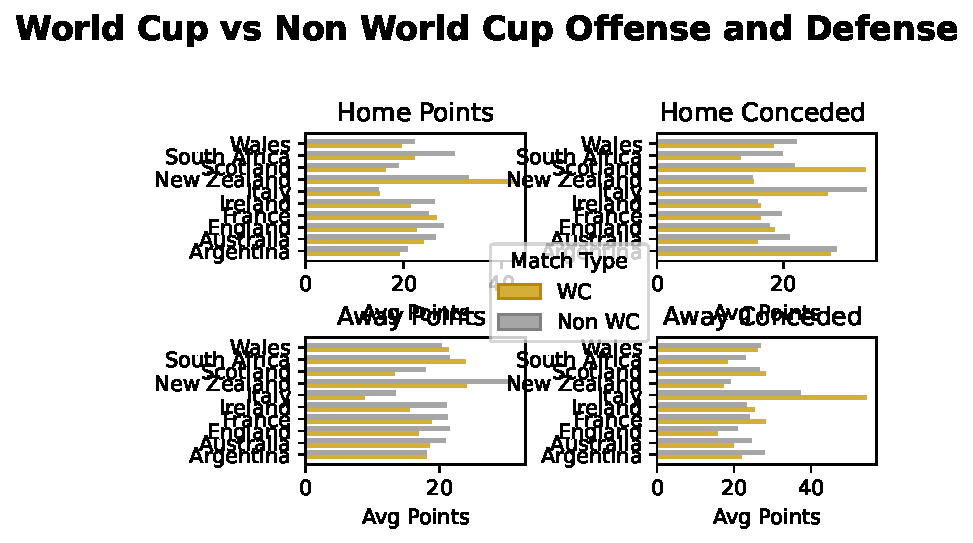
\includegraphics[keepaspectratio]{Preliminary Analysis_files/figure-pdf/cell-11-output-1.pdf}}
::: ::: \\
\textbf{4. Year-wise Win Percentage Trends} - Shows \textbf{consistency
and peaks} for contenders like \textbf{NZ, RSA, and IRE}. - Allows
modeling team form trajectory over time. \\
::: \{.cell execution\_count=11\} ``` \{.python .cell-code\} \#only kees
the year, awayWin, homeWin, and country year\_wise =
rugbyDF{[}{[}``home\_team'',``away\_team'',``homeWin'',``awayWin'',``count'',``year''{]}{]} \\
\#drops the away in homeDf and home in awayDf home\_year\_wise =
year\_wise.drop(columns=\{``away\_team'',``awayWin''\}) away\_year\_wise
= year\_wise.drop(columns=\{``home\_team'',``homeWin''\}) \\
\#renames so that both df have the same col names for concatenation
home\_year\_wise =
home\_year\_wise.rename(columns=\{``home\_team'':``team'',``homeWin'':``win''\})
away\_year\_wise =
away\_year\_wise.rename(columns=\{``away\_team'':``team'',``awayWin'':``win''\})
year\_wise = pd.concat({[}home\_year\_wise,away\_year\_wise{]},
axis=0).reset\_index(drop=True) \\
\#groups the data by year and by team and then cerates a win\% col for
normalized results def getGroupedYW(year\_wise): year\_wise\_grouped =
year\_wise.groupby({[}``team'',``year''{]}).sum()
year\_wise\_grouped{[}``win\_\%''{]} =
year\_wise\_grouped{[}``win''{]}.div(year\_wise\_grouped{[}``count''{]})*100
year\_wise\_grouped =
year\_wise\_grouped.drop(columns=\{``win'',``count''\}) return
year\_wise\_grouped \\
year\_wise\_grouped = getGroupedYW(year\_wise) ``` ::: \\
::: \{.cell execution\_count=12\} ``` \{.python .cell-code\} def
plotYearWiseData(year\_wise\_grouped): year\_wise\_grouped\_reset =
year\_wise\_grouped.reset\_index() \\
plt.figure(figsize=(7.5, 5))
sns.lineplot(data=year\_wise\_grouped\_reset, x=`year', y=`win\_\%',
hue=`team', style=`team', markers=True, dashes=False) \\
plt.title(`Win Percentage by Team Over the Years') plt.xlabel(`Year')
plt.ylabel(`Win Percentage') plt.legend(bbox\_to\_anchor=(1.001, 1),
loc=`upper left') plt.grid(True) plt.tight\_layout() plt.show()
plt.close() \\
plotYearWiseData(year\_wise\_grouped) ``` \\
::: \{.cell-output .cell-output-display\}
\pandocbounded{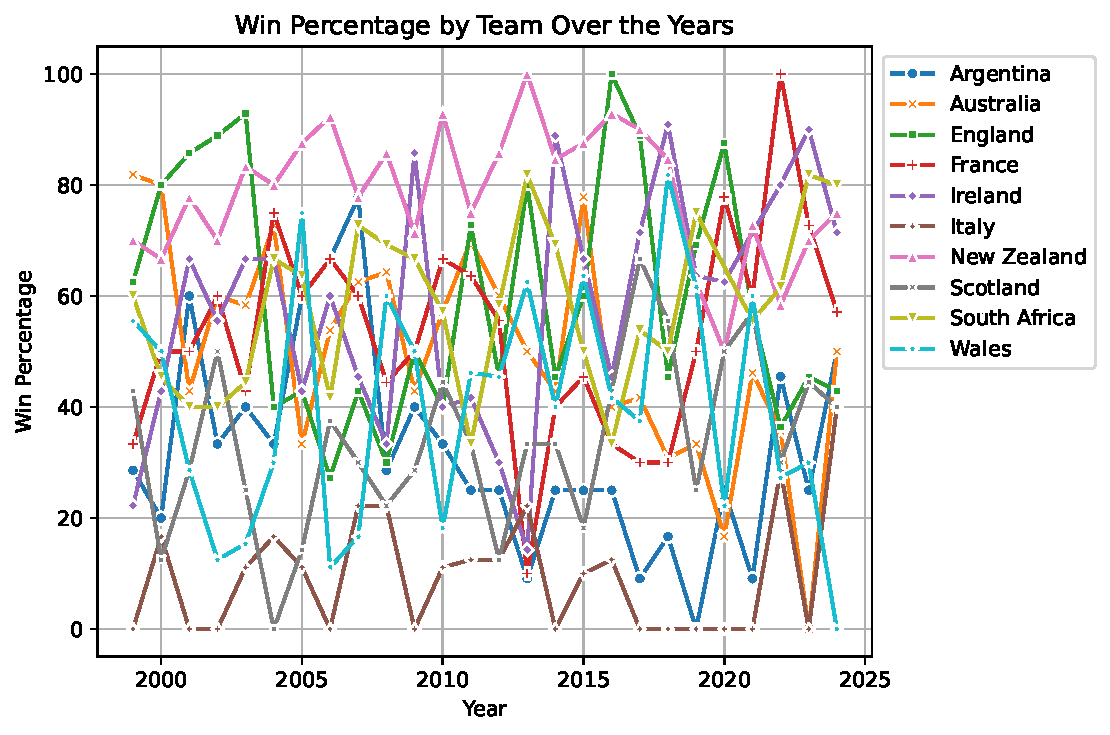
\includegraphics[keepaspectratio]{Preliminary Analysis_files/figure-pdf/cell-13-output-1.pdf}}
::: ::: \\
Since this plot is chaotic, I will cut down on the number of countries
plotted. 2 plots with 5 countries on each. \\
::: \{.cell execution\_count=13\} ``` \{.python .cell-code\} \# Split
teams into two halves half\_idx = len(unq\_teams) // 2
first\_half\_teams = unq\_teams{[}:half\_idx{]} second\_half\_teams =
unq\_teams{[}half\_idx:{]} \\
\# Create filtered DataFrames df\_first\_half =
year\_wise{[}year\_wise{[}`team'{]}.isin(first\_half\_teams){]}
df\_second\_half =
year\_wise{[}year\_wise{[}`team'{]}.isin(second\_half\_teams){]} \\
\#Checking if the teams do not overlap
df\_first\_half{[}``team''{]}.unique()
df\_second\_half{[}``team''{]}.unique() ``` \\
::: \{.cell-output .cell-output-display execution\_count=13\} \\
::: \{.cell execution\_count=14\} ``` \{.python .cell-code\} \#uses the
function to create the grouped data first\_half\_grouped =
getGroupedYW(df\_first\_half) \\
\#plots it plotYearWiseData(first\_half\_grouped) ``` \\
::: \{.cell-output .cell-output-display\}
\pandocbounded{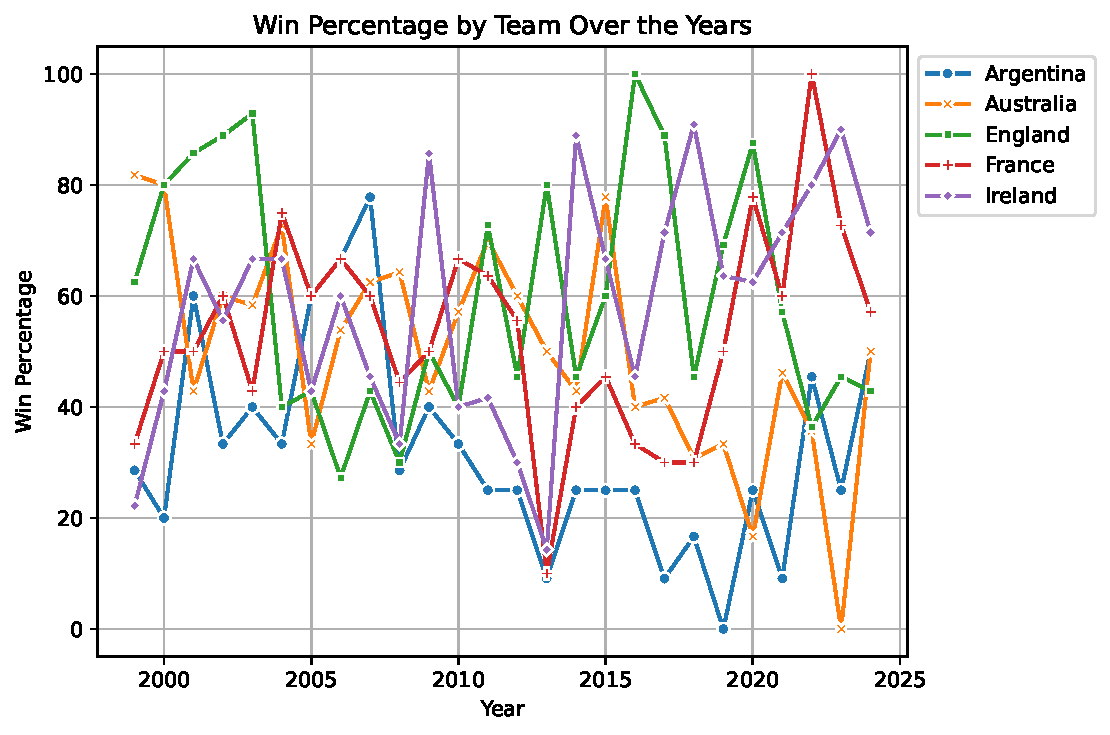
\includegraphics[keepaspectratio]{Preliminary Analysis_files/figure-pdf/cell-15-output-1.pdf}}
::: ::: \\
In this breakdown of ARG, AUS, ENG, FRA, and IRE we can see that
Australia starts out really strong at the turn of the millennium and
slowly starts to regress. 2023 saw them experience their worst year with
no wins to show for. IRE and FRA have been the two teams that continue
to improve on average. ENG and ARG are the two wildcard teams that can
be either really good or really bad; they are wildly unpredictable. \\
::: \{.cell execution\_count=15\} ``` \{.python .cell-code\} \#uses the
function to create the grouped data second\_half\_grouped =
getGroupedYW(df\_second\_half) \\
\#plots it plotYearWiseData(second\_half\_grouped) ``` \\
::: \{.cell-output .cell-output-display\}
\pandocbounded{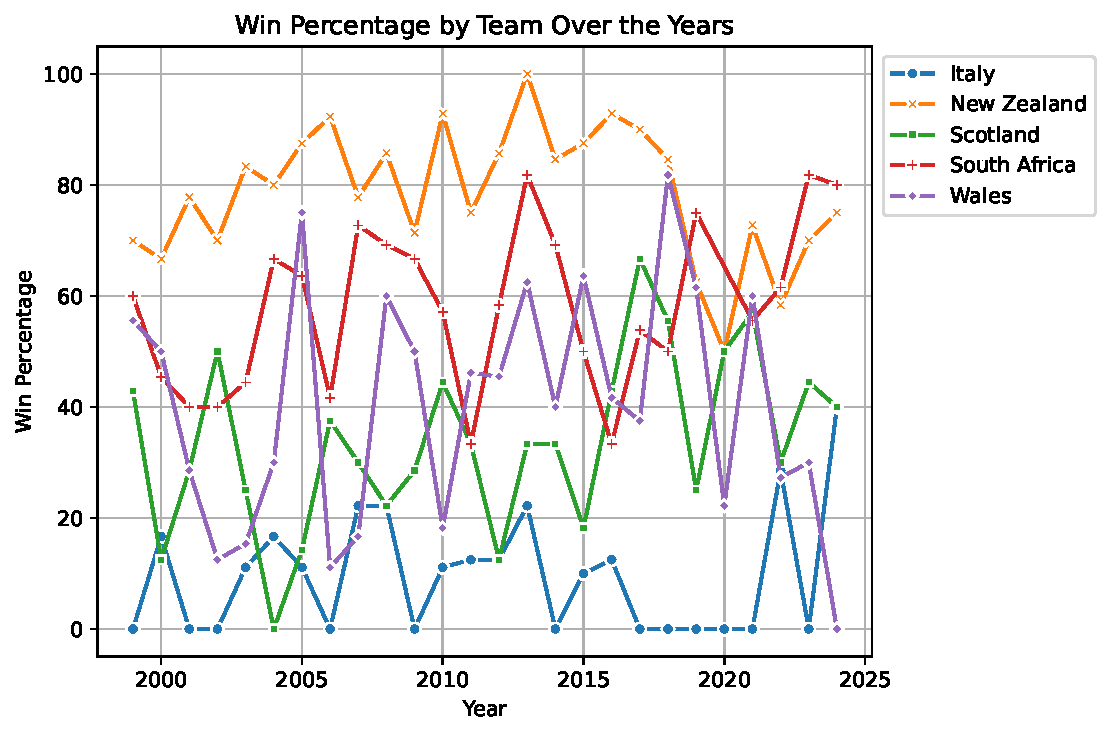
\includegraphics[keepaspectratio]{Preliminary Analysis_files/figure-pdf/cell-16-output-1.pdf}}
::: ::: \\
\end{longtable}

\subsubsection{\texorpdfstring{\textbf{Modeling
Approach}}{Modeling Approach}}\label{modeling-approach}

\paragraph{\texorpdfstring{\textbf{Random Forest
Classifier}}{Random Forest Classifier}}\label{random-forest-classifier}

\begin{itemize}
\tightlist
\item
  Used for \textbf{binary classification}: World Cup Winner
  vs.~Non-Winner.
\item
  Captures \textbf{non-linear patterns} and \textbf{interaction
  effects}.
\item
  Feature importance helps identify key performance indicators.
\end{itemize}

\paragraph{\texorpdfstring{\textbf{Time-Series
Analysis}}{Time-Series Analysis}}\label{time-series-analysis}

\begin{itemize}
\tightlist
\item
  Year-wise win percentage trends inform about \textbf{form, slumps, and
  growth}.
\item
  Useful for \textbf{pre-tournament prediction}, especially for 2027.
\end{itemize}

\begin{center}\rule{0.5\linewidth}{0.5pt}\end{center}

\subsubsection{\texorpdfstring{\textbf{Why These
Methods?}}{Why These Methods?}}\label{why-these-methods}

\begin{itemize}
\tightlist
\item
  \textbf{Logistic regression} works well with ordered categories.
\item
  \textbf{Random forests} are robust to outliers and handle complex
  variable relationships.
\item
  \textbf{Visualization-backed wrangling} ensured each model was driven
  by interpretable and meaningful variables.
\end{itemize}

\begin{center}\rule{0.5\linewidth}{0.5pt}\end{center}

\paragraph{\texorpdfstring{\textbf{XGBoost CLassifier with Monte Carlo
Simulations}}{XGBoost CLassifier with Monte Carlo Simulations}}\label{xgboost-classifier-with-monte-carlo-simulations}

XGBoost (Extreme Gradient Boosting) is a highly efficient and scalable
machine learning algorithm, especially for structured/tabular data. Its
advantages include:

\begin{itemize}
\item
  High Predictive Accuracy: Often outperforms other algorithms (like
  logistic regression, random forests, or neural networks) on structured
  datasets.
\item
  Handles Non-Linearity \& Complex Relationships: Captures intricate
  patterns in data that simpler models might miss.
\item
  Feature Importance: Provides insights into which variables most
  influence predictions.
\item
  Robust to Overfitting: Includes regularization (L1/L2) and early
  stopping.
\item
  Works Well with Imbalanced Data: Can handle classification tasks where
  one class is rare (e.g., fraud detection).
\end{itemize}

Monte Carlo (MC) simulations are used to model uncertainty and
probabilistic outcomes by running thousands of random simulations. When
combined with XGBoost, they help:

\begin{itemize}
\item
  Quantify Uncertainty: XGBoost gives a point prediction (e.g.,
  probability of an event), but MC can simulate how reliable that
  prediction is under varying conditions.
\item
  Risk Assessment: If inputs have randomness (e.g., stock prices, sensor
  noise), MC can propagate this uncertainty through the XGBoost model.
\item
  Sensitivity Analysis: Test how small changes in input variables affect
  the output (e.g., ``What if Feature X varies by ±10\%?'').
\item
  Decision-Making Under Uncertainty: Useful in finance (portfolio risk),
  healthcare (treatment outcomes), or engineering (system failures).
\end{itemize}

\begin{Shaded}
\begin{Highlighting}[]
\CommentTok{\# Load the dataset}
\NormalTok{df }\OperatorTok{=}\NormalTok{ pd.read\_csv(}\StringTok{\textquotesingle{}data/rugby.csv\textquotesingle{}}\NormalTok{)}
\NormalTok{df[}\StringTok{\textquotesingle{}year\textquotesingle{}}\NormalTok{] }\OperatorTok{=}\NormalTok{ df[}\StringTok{\textquotesingle{}date\textquotesingle{}}\NormalTok{].}\BuiltInTok{str}\NormalTok{[}\DecValTok{0}\NormalTok{:}\DecValTok{4}\NormalTok{].astype(}\BuiltInTok{int}\NormalTok{)}
\NormalTok{df }\OperatorTok{=}\NormalTok{ df[df.year }\OperatorTok{\textgreater{}} \DecValTok{1998}\NormalTok{]}
\CommentTok{\# Data preprocessing}
\CommentTok{\# Filter to only international matches (remove club matches)}
\NormalTok{international\_matches }\OperatorTok{=}\NormalTok{ df[}\StringTok{\textquotesingle{}competition\textquotesingle{}}\NormalTok{].}\BuiltInTok{str}\NormalTok{.contains(}\StringTok{\textquotesingle{}International|Championship|Nations|World Cup|Test Match\textquotesingle{}}\NormalTok{, na}\OperatorTok{=}\VariableTok{False}\NormalTok{)}
\NormalTok{df }\OperatorTok{=}\NormalTok{ df.loc[international\_matches].copy()}

\CommentTok{\# Feature engineering}
\CommentTok{\# Create target variable {-} winner of each match}
\NormalTok{conditions }\OperatorTok{=}\NormalTok{ [}
\NormalTok{    df[}\StringTok{\textquotesingle{}home\_score\textquotesingle{}}\NormalTok{] }\OperatorTok{\textgreater{}}\NormalTok{ df[}\StringTok{\textquotesingle{}away\_score\textquotesingle{}}\NormalTok{],}
\NormalTok{    df[}\StringTok{\textquotesingle{}home\_score\textquotesingle{}}\NormalTok{] }\OperatorTok{\textless{}}\NormalTok{ df[}\StringTok{\textquotesingle{}away\_score\textquotesingle{}}\NormalTok{]}
\NormalTok{]}
\NormalTok{choices }\OperatorTok{=}\NormalTok{ [df[}\StringTok{\textquotesingle{}home\_team\textquotesingle{}}\NormalTok{], df[}\StringTok{\textquotesingle{}away\_team\textquotesingle{}}\NormalTok{]]}
\NormalTok{df.loc[:, }\StringTok{\textquotesingle{}winner\textquotesingle{}}\NormalTok{] }\OperatorTok{=}\NormalTok{ np.select(conditions, choices, default}\OperatorTok{=}\StringTok{\textquotesingle{}Draw\textquotesingle{}}\NormalTok{)}

\CommentTok{\# Remove draws for classification}
\NormalTok{df }\OperatorTok{=}\NormalTok{ df.loc[df[}\StringTok{\textquotesingle{}winner\textquotesingle{}}\NormalTok{] }\OperatorTok{!=} \StringTok{\textquotesingle{}Draw\textquotesingle{}}\NormalTok{].copy()}

\CommentTok{\# Encode categorical variables}
\NormalTok{le }\OperatorTok{=}\NormalTok{ LabelEncoder()}
\NormalTok{df.loc[:, }\StringTok{\textquotesingle{}home\_team\_encoded\textquotesingle{}}\NormalTok{] }\OperatorTok{=}\NormalTok{ le.fit\_transform(df[}\StringTok{\textquotesingle{}home\_team\textquotesingle{}}\NormalTok{])}
\NormalTok{df.loc[:, }\StringTok{\textquotesingle{}away\_team\_encoded\textquotesingle{}}\NormalTok{] }\OperatorTok{=}\NormalTok{ le.transform(df[}\StringTok{\textquotesingle{}away\_team\textquotesingle{}}\NormalTok{])}
\NormalTok{df.loc[:, }\StringTok{\textquotesingle{}winner\_encoded\textquotesingle{}}\NormalTok{] }\OperatorTok{=}\NormalTok{ le.transform(df[}\StringTok{\textquotesingle{}winner\textquotesingle{}}\NormalTok{])}

\CommentTok{\# Create features based on historical performance}
\KeywordTok{def}\NormalTok{ calculate\_team\_stats(df):}
\NormalTok{    team\_stats }\OperatorTok{=}\NormalTok{ defaultdict(}\KeywordTok{lambda}\NormalTok{: \{}\StringTok{\textquotesingle{}games\textquotesingle{}}\NormalTok{: }\DecValTok{0}\NormalTok{, }\StringTok{\textquotesingle{}wins\textquotesingle{}}\NormalTok{: }\DecValTok{0}\NormalTok{, }\StringTok{\textquotesingle{}points\_for\textquotesingle{}}\NormalTok{: }\DecValTok{0}\NormalTok{, }\StringTok{\textquotesingle{}points\_against\textquotesingle{}}\NormalTok{: }\DecValTok{0}\NormalTok{\})}
    
    \ControlFlowTok{for}\NormalTok{ \_, row }\KeywordTok{in}\NormalTok{ df.iterrows():}
\NormalTok{        home\_team }\OperatorTok{=}\NormalTok{ row[}\StringTok{\textquotesingle{}home\_team\textquotesingle{}}\NormalTok{]}
\NormalTok{        away\_team }\OperatorTok{=}\NormalTok{ row[}\StringTok{\textquotesingle{}away\_team\textquotesingle{}}\NormalTok{]}
\NormalTok{        home\_score }\OperatorTok{=}\NormalTok{ row[}\StringTok{\textquotesingle{}home\_score\textquotesingle{}}\NormalTok{]}
\NormalTok{        away\_score }\OperatorTok{=}\NormalTok{ row[}\StringTok{\textquotesingle{}away\_score\textquotesingle{}}\NormalTok{]}
        
        \CommentTok{\# Update home team stats}
\NormalTok{        team\_stats[home\_team][}\StringTok{\textquotesingle{}games\textquotesingle{}}\NormalTok{] }\OperatorTok{+=} \DecValTok{1}
\NormalTok{        team\_stats[home\_team][}\StringTok{\textquotesingle{}points\_for\textquotesingle{}}\NormalTok{] }\OperatorTok{+=}\NormalTok{ home\_score}
\NormalTok{        team\_stats[home\_team][}\StringTok{\textquotesingle{}points\_against\textquotesingle{}}\NormalTok{] }\OperatorTok{+=}\NormalTok{ away\_score}
\NormalTok{        team\_stats[home\_team][}\StringTok{\textquotesingle{}wins\textquotesingle{}}\NormalTok{] }\OperatorTok{+=} \DecValTok{1} \ControlFlowTok{if}\NormalTok{ home\_score }\OperatorTok{\textgreater{}}\NormalTok{ away\_score }\ControlFlowTok{else} \DecValTok{0}
        
        \CommentTok{\# Update away team stats}
\NormalTok{        team\_stats[away\_team][}\StringTok{\textquotesingle{}games\textquotesingle{}}\NormalTok{] }\OperatorTok{+=} \DecValTok{1}
\NormalTok{        team\_stats[away\_team][}\StringTok{\textquotesingle{}points\_for\textquotesingle{}}\NormalTok{] }\OperatorTok{+=}\NormalTok{ away\_score}
\NormalTok{        team\_stats[away\_team][}\StringTok{\textquotesingle{}points\_against\textquotesingle{}}\NormalTok{] }\OperatorTok{+=}\NormalTok{ home\_score}
\NormalTok{        team\_stats[away\_team][}\StringTok{\textquotesingle{}wins\textquotesingle{}}\NormalTok{] }\OperatorTok{+=} \DecValTok{1} \ControlFlowTok{if}\NormalTok{ away\_score }\OperatorTok{\textgreater{}}\NormalTok{ home\_score }\ControlFlowTok{else} \DecValTok{0}
    
    \ControlFlowTok{return}\NormalTok{ team\_stats}

\CommentTok{\# Calculate rolling stats}
\NormalTok{team\_stats }\OperatorTok{=}\NormalTok{ calculate\_team\_stats(df)}

\CommentTok{\# Add features to dataframe}
\KeywordTok{def}\NormalTok{ add\_features(df, team\_stats):}
\NormalTok{    df }\OperatorTok{=}\NormalTok{ df.copy()}
\NormalTok{    df.loc[:, }\StringTok{\textquotesingle{}home\_win\_pct\textquotesingle{}}\NormalTok{] }\OperatorTok{=}\NormalTok{ df[}\StringTok{\textquotesingle{}home\_team\textquotesingle{}}\NormalTok{].}\BuiltInTok{apply}\NormalTok{(}
        \KeywordTok{lambda}\NormalTok{ x: team\_stats[x][}\StringTok{\textquotesingle{}wins\textquotesingle{}}\NormalTok{] }\OperatorTok{/}\NormalTok{ team\_stats[x][}\StringTok{\textquotesingle{}games\textquotesingle{}}\NormalTok{] }\ControlFlowTok{if}\NormalTok{ team\_stats[x][}\StringTok{\textquotesingle{}games\textquotesingle{}}\NormalTok{] }\OperatorTok{\textgreater{}} \DecValTok{0} \ControlFlowTok{else} \FloatTok{0.5}\NormalTok{)}
\NormalTok{    df.loc[:, }\StringTok{\textquotesingle{}away\_win\_pct\textquotesingle{}}\NormalTok{] }\OperatorTok{=}\NormalTok{ df[}\StringTok{\textquotesingle{}away\_team\textquotesingle{}}\NormalTok{].}\BuiltInTok{apply}\NormalTok{(}
        \KeywordTok{lambda}\NormalTok{ x: team\_stats[x][}\StringTok{\textquotesingle{}wins\textquotesingle{}}\NormalTok{] }\OperatorTok{/}\NormalTok{ team\_stats[x][}\StringTok{\textquotesingle{}games\textquotesingle{}}\NormalTok{] }\ControlFlowTok{if}\NormalTok{ team\_stats[x][}\StringTok{\textquotesingle{}games\textquotesingle{}}\NormalTok{] }\OperatorTok{\textgreater{}} \DecValTok{0} \ControlFlowTok{else} \FloatTok{0.5}\NormalTok{)}
\NormalTok{    df.loc[:, }\StringTok{\textquotesingle{}home\_points\_avg\textquotesingle{}}\NormalTok{] }\OperatorTok{=}\NormalTok{ df[}\StringTok{\textquotesingle{}home\_team\textquotesingle{}}\NormalTok{].}\BuiltInTok{apply}\NormalTok{(}
        \KeywordTok{lambda}\NormalTok{ x: team\_stats[x][}\StringTok{\textquotesingle{}points\_for\textquotesingle{}}\NormalTok{] }\OperatorTok{/}\NormalTok{ team\_stats[x][}\StringTok{\textquotesingle{}games\textquotesingle{}}\NormalTok{] }\ControlFlowTok{if}\NormalTok{ team\_stats[x][}\StringTok{\textquotesingle{}games\textquotesingle{}}\NormalTok{] }\OperatorTok{\textgreater{}} \DecValTok{0} \ControlFlowTok{else} \DecValTok{0}\NormalTok{)}
\NormalTok{    df.loc[:, }\StringTok{\textquotesingle{}away\_points\_avg\textquotesingle{}}\NormalTok{] }\OperatorTok{=}\NormalTok{ df[}\StringTok{\textquotesingle{}away\_team\textquotesingle{}}\NormalTok{].}\BuiltInTok{apply}\NormalTok{(}
        \KeywordTok{lambda}\NormalTok{ x: team\_stats[x][}\StringTok{\textquotesingle{}points\_for\textquotesingle{}}\NormalTok{] }\OperatorTok{/}\NormalTok{ team\_stats[x][}\StringTok{\textquotesingle{}games\textquotesingle{}}\NormalTok{] }\ControlFlowTok{if}\NormalTok{ team\_stats[x][}\StringTok{\textquotesingle{}games\textquotesingle{}}\NormalTok{] }\OperatorTok{\textgreater{}} \DecValTok{0} \ControlFlowTok{else} \DecValTok{0}\NormalTok{)}
\NormalTok{    df.loc[:, }\StringTok{\textquotesingle{}home\_points\_against\_avg\textquotesingle{}}\NormalTok{] }\OperatorTok{=}\NormalTok{ df[}\StringTok{\textquotesingle{}home\_team\textquotesingle{}}\NormalTok{].}\BuiltInTok{apply}\NormalTok{(}
        \KeywordTok{lambda}\NormalTok{ x: team\_stats[x][}\StringTok{\textquotesingle{}points\_against\textquotesingle{}}\NormalTok{] }\OperatorTok{/}\NormalTok{ team\_stats[x][}\StringTok{\textquotesingle{}games\textquotesingle{}}\NormalTok{] }\ControlFlowTok{if}\NormalTok{ team\_stats[x][}\StringTok{\textquotesingle{}games\textquotesingle{}}\NormalTok{] }\OperatorTok{\textgreater{}} \DecValTok{0} \ControlFlowTok{else} \DecValTok{0}\NormalTok{)}
\NormalTok{    df.loc[:, }\StringTok{\textquotesingle{}away\_points\_against\_avg\textquotesingle{}}\NormalTok{] }\OperatorTok{=}\NormalTok{ df[}\StringTok{\textquotesingle{}away\_team\textquotesingle{}}\NormalTok{].}\BuiltInTok{apply}\NormalTok{(}
        \KeywordTok{lambda}\NormalTok{ x: team\_stats[x][}\StringTok{\textquotesingle{}points\_against\textquotesingle{}}\NormalTok{] }\OperatorTok{/}\NormalTok{ team\_stats[x][}\StringTok{\textquotesingle{}games\textquotesingle{}}\NormalTok{] }\ControlFlowTok{if}\NormalTok{ team\_stats[x][}\StringTok{\textquotesingle{}games\textquotesingle{}}\NormalTok{] }\OperatorTok{\textgreater{}} \DecValTok{0} \ControlFlowTok{else} \DecValTok{0}\NormalTok{)}
    
    \CommentTok{\# Add some interaction features}
\NormalTok{    df.loc[:, }\StringTok{\textquotesingle{}win\_pct\_diff\textquotesingle{}}\NormalTok{] }\OperatorTok{=}\NormalTok{ df[}\StringTok{\textquotesingle{}home\_win\_pct\textquotesingle{}}\NormalTok{] }\OperatorTok{{-}}\NormalTok{ df[}\StringTok{\textquotesingle{}away\_win\_pct\textquotesingle{}}\NormalTok{]}
\NormalTok{    df.loc[:, }\StringTok{\textquotesingle{}points\_diff\textquotesingle{}}\NormalTok{] }\OperatorTok{=}\NormalTok{ df[}\StringTok{\textquotesingle{}home\_points\_avg\textquotesingle{}}\NormalTok{] }\OperatorTok{{-}}\NormalTok{ df[}\StringTok{\textquotesingle{}away\_points\_avg\textquotesingle{}}\NormalTok{]}
    
    \ControlFlowTok{return}\NormalTok{ df}

\NormalTok{df }\OperatorTok{=}\NormalTok{ add\_features(df, team\_stats)}
\end{Highlighting}
\end{Shaded}

\begin{Shaded}
\begin{Highlighting}[]
\CommentTok{\# Split into features and target}
\NormalTok{feature\_cols }\OperatorTok{=}\NormalTok{ [}\StringTok{\textquotesingle{}home\_team\_encoded\textquotesingle{}}\NormalTok{, }\StringTok{\textquotesingle{}away\_team\_encoded\textquotesingle{}}\NormalTok{, }
                \StringTok{\textquotesingle{}home\_win\_pct\textquotesingle{}}\NormalTok{, }\StringTok{\textquotesingle{}away\_win\_pct\textquotesingle{}}\NormalTok{, }
                \StringTok{\textquotesingle{}home\_points\_avg\textquotesingle{}}\NormalTok{, }\StringTok{\textquotesingle{}away\_points\_avg\textquotesingle{}}\NormalTok{,}
                \StringTok{\textquotesingle{}home\_points\_against\_avg\textquotesingle{}}\NormalTok{, }\StringTok{\textquotesingle{}away\_points\_against\_avg\textquotesingle{}}\NormalTok{,}
                \StringTok{\textquotesingle{}win\_pct\_diff\textquotesingle{}}\NormalTok{, }\StringTok{\textquotesingle{}points\_diff\textquotesingle{}}\NormalTok{]}
\NormalTok{X }\OperatorTok{=}\NormalTok{ df.loc[:, feature\_cols]}
\NormalTok{y }\OperatorTok{=}\NormalTok{ df.loc[:, }\StringTok{\textquotesingle{}winner\_encoded\textquotesingle{}}\NormalTok{]}

\CommentTok{\# Split into train and test sets}
\NormalTok{X\_train, X\_test, y\_train, y\_test }\OperatorTok{=}\NormalTok{ train\_test\_split(X, y, test\_size}\OperatorTok{=}\FloatTok{0.2}\NormalTok{, random\_state}\OperatorTok{=}\DecValTok{42}\NormalTok{)}

\CommentTok{\# Train XGBoost model}
\NormalTok{model }\OperatorTok{=}\NormalTok{ xgb.XGBClassifier(}
\NormalTok{    objective}\OperatorTok{=}\StringTok{\textquotesingle{}multi:softprob\textquotesingle{}}\NormalTok{,}
\NormalTok{    num\_class}\OperatorTok{=}\BuiltInTok{len}\NormalTok{(le.classes\_),}
\NormalTok{    n\_estimators}\OperatorTok{=}\DecValTok{100}\NormalTok{,}
\NormalTok{    max\_depth}\OperatorTok{=}\DecValTok{5}\NormalTok{,}
\NormalTok{    learning\_rate}\OperatorTok{=}\FloatTok{0.1}\NormalTok{,}
\NormalTok{    random\_state}\OperatorTok{=}\DecValTok{42}
\NormalTok{)}

\NormalTok{model.fit(X\_train, y\_train)}

\CommentTok{\# Evaluate model}
\NormalTok{y\_pred }\OperatorTok{=}\NormalTok{ model.predict(X\_test)}
\NormalTok{accuracy }\OperatorTok{=}\NormalTok{ accuracy\_score(y\_test, y\_pred)}
\BuiltInTok{print}\NormalTok{(}\SpecialStringTok{f"Model accuracy: }\SpecialCharTok{\{}\NormalTok{accuracy}\SpecialCharTok{:.2f\}}\SpecialStringTok{"}\NormalTok{)}
\end{Highlighting}
\end{Shaded}

\begin{verbatim}
Model accuracy: 0.78
\end{verbatim}

\begin{Shaded}
\begin{Highlighting}[]
\CommentTok{\# Monte Carlo simulation for World Cup prediction}
\KeywordTok{def}\NormalTok{ simulate\_world\_cup(teams, model, le, n\_simulations}\OperatorTok{=}\DecValTok{1000}\NormalTok{):}
    \CommentTok{\# Get current top teams (from our dataset)}
\NormalTok{    top\_teams }\OperatorTok{=}\NormalTok{ [}\StringTok{\textquotesingle{}New Zealand\textquotesingle{}}\NormalTok{, }\StringTok{\textquotesingle{}South Africa\textquotesingle{}}\NormalTok{, }\StringTok{\textquotesingle{}Australia\textquotesingle{}}\NormalTok{, }\StringTok{\textquotesingle{}England\textquotesingle{}}\NormalTok{, }\StringTok{\textquotesingle{}France\textquotesingle{}}\NormalTok{, }
                 \StringTok{\textquotesingle{}Ireland\textquotesingle{}}\NormalTok{, }\StringTok{\textquotesingle{}Wales\textquotesingle{}}\NormalTok{, }\StringTok{\textquotesingle{}Scotland\textquotesingle{}}\NormalTok{, }\StringTok{\textquotesingle{}Argentina\textquotesingle{}}\NormalTok{, }\StringTok{\textquotesingle{}Italy\textquotesingle{}}\NormalTok{]}
    
    \CommentTok{\# Create a dictionary to store win counts}
\NormalTok{    win\_counts }\OperatorTok{=}\NormalTok{ \{team: }\DecValTok{0} \ControlFlowTok{for}\NormalTok{ team }\KeywordTok{in}\NormalTok{ top\_teams\}}
    
    \ControlFlowTok{for}\NormalTok{ \_ }\KeywordTok{in} \BuiltInTok{range}\NormalTok{(n\_simulations):}
        \CommentTok{\# Randomly select 2 teams to "play" in the final}
\NormalTok{        finalists }\OperatorTok{=}\NormalTok{ random.sample(top\_teams, }\DecValTok{2}\NormalTok{)}
\NormalTok{        team1, team2 }\OperatorTok{=}\NormalTok{ finalists}
        
        \CommentTok{\# Create feature vector for this matchup}
        \ControlFlowTok{try}\NormalTok{:}
\NormalTok{            team1\_encoded }\OperatorTok{=}\NormalTok{ le.transform([team1])[}\DecValTok{0}\NormalTok{]}
\NormalTok{            team2\_encoded }\OperatorTok{=}\NormalTok{ le.transform([team2])[}\DecValTok{0}\NormalTok{]}
        \ControlFlowTok{except} \PreprocessorTok{ValueError}\NormalTok{:}
            \CommentTok{\# Skip if team not in our training data}
            \ControlFlowTok{continue}
            
        \CommentTok{\# Get team stats (simplified {-} in practice you\textquotesingle{}d want more recent stats)}
\NormalTok{        team1\_stats }\OperatorTok{=}\NormalTok{ team\_stats.get(team1, \{}\StringTok{\textquotesingle{}games\textquotesingle{}}\NormalTok{: }\DecValTok{1}\NormalTok{, }\StringTok{\textquotesingle{}wins\textquotesingle{}}\NormalTok{: }\DecValTok{0}\NormalTok{, }\StringTok{\textquotesingle{}points\_for\textquotesingle{}}\NormalTok{: }\DecValTok{0}\NormalTok{, }\StringTok{\textquotesingle{}points\_against\textquotesingle{}}\NormalTok{: }\DecValTok{0}\NormalTok{\})}
\NormalTok{        team2\_stats }\OperatorTok{=}\NormalTok{ team\_stats.get(team2, \{}\StringTok{\textquotesingle{}games\textquotesingle{}}\NormalTok{: }\DecValTok{1}\NormalTok{, }\StringTok{\textquotesingle{}wins\textquotesingle{}}\NormalTok{: }\DecValTok{0}\NormalTok{, }\StringTok{\textquotesingle{}points\_for\textquotesingle{}}\NormalTok{: }\DecValTok{0}\NormalTok{, }\StringTok{\textquotesingle{}points\_against\textquotesingle{}}\NormalTok{: }\DecValTok{0}\NormalTok{\})}
        
        \CommentTok{\# Create feature row}
\NormalTok{        features }\OperatorTok{=}\NormalTok{ np.array([}
\NormalTok{            team1\_encoded, team2\_encoded,}
\NormalTok{            team1\_stats[}\StringTok{\textquotesingle{}wins\textquotesingle{}}\NormalTok{] }\OperatorTok{/} \BuiltInTok{max}\NormalTok{(}\DecValTok{1}\NormalTok{, team1\_stats[}\StringTok{\textquotesingle{}games\textquotesingle{}}\NormalTok{]),}
\NormalTok{            team2\_stats[}\StringTok{\textquotesingle{}wins\textquotesingle{}}\NormalTok{] }\OperatorTok{/} \BuiltInTok{max}\NormalTok{(}\DecValTok{1}\NormalTok{, team2\_stats[}\StringTok{\textquotesingle{}games\textquotesingle{}}\NormalTok{]),}
\NormalTok{            team1\_stats[}\StringTok{\textquotesingle{}points\_for\textquotesingle{}}\NormalTok{] }\OperatorTok{/} \BuiltInTok{max}\NormalTok{(}\DecValTok{1}\NormalTok{, team1\_stats[}\StringTok{\textquotesingle{}games\textquotesingle{}}\NormalTok{]),}
\NormalTok{            team2\_stats[}\StringTok{\textquotesingle{}points\_for\textquotesingle{}}\NormalTok{] }\OperatorTok{/} \BuiltInTok{max}\NormalTok{(}\DecValTok{1}\NormalTok{, team2\_stats[}\StringTok{\textquotesingle{}games\textquotesingle{}}\NormalTok{]),}
\NormalTok{            team1\_stats[}\StringTok{\textquotesingle{}points\_against\textquotesingle{}}\NormalTok{] }\OperatorTok{/} \BuiltInTok{max}\NormalTok{(}\DecValTok{1}\NormalTok{, team1\_stats[}\StringTok{\textquotesingle{}games\textquotesingle{}}\NormalTok{]),}
\NormalTok{            team2\_stats[}\StringTok{\textquotesingle{}points\_against\textquotesingle{}}\NormalTok{] }\OperatorTok{/} \BuiltInTok{max}\NormalTok{(}\DecValTok{1}\NormalTok{, team2\_stats[}\StringTok{\textquotesingle{}games\textquotesingle{}}\NormalTok{]),}
\NormalTok{            (team1\_stats[}\StringTok{\textquotesingle{}wins\textquotesingle{}}\NormalTok{] }\OperatorTok{/} \BuiltInTok{max}\NormalTok{(}\DecValTok{1}\NormalTok{, team1\_stats[}\StringTok{\textquotesingle{}games\textquotesingle{}}\NormalTok{])) }\OperatorTok{{-}} 
\NormalTok{            (team2\_stats[}\StringTok{\textquotesingle{}wins\textquotesingle{}}\NormalTok{] }\OperatorTok{/} \BuiltInTok{max}\NormalTok{(}\DecValTok{1}\NormalTok{, team2\_stats[}\StringTok{\textquotesingle{}games\textquotesingle{}}\NormalTok{])),}
\NormalTok{            (team1\_stats[}\StringTok{\textquotesingle{}points\_for\textquotesingle{}}\NormalTok{] }\OperatorTok{/} \BuiltInTok{max}\NormalTok{(}\DecValTok{1}\NormalTok{, team1\_stats[}\StringTok{\textquotesingle{}games\textquotesingle{}}\NormalTok{])) }\OperatorTok{{-}} 
\NormalTok{            (team2\_stats[}\StringTok{\textquotesingle{}points\_for\textquotesingle{}}\NormalTok{] }\OperatorTok{/} \BuiltInTok{max}\NormalTok{(}\DecValTok{1}\NormalTok{, team2\_stats[}\StringTok{\textquotesingle{}games\textquotesingle{}}\NormalTok{]))}
\NormalTok{        ]).reshape(}\DecValTok{1}\NormalTok{, }\OperatorTok{{-}}\DecValTok{1}\NormalTok{)}
        
        \CommentTok{\# Predict probabilities}
        \ControlFlowTok{try}\NormalTok{:}
\NormalTok{            probs }\OperatorTok{=}\NormalTok{ model.predict\_proba(features)[}\DecValTok{0}\NormalTok{]}
            
            \CommentTok{\# Sample winner based on probabilities}
\NormalTok{            winner\_idx }\OperatorTok{=}\NormalTok{ np.random.choice(}\BuiltInTok{len}\NormalTok{(probs), p}\OperatorTok{=}\NormalTok{probs)}
\NormalTok{            winner }\OperatorTok{=}\NormalTok{ le.inverse\_transform([winner\_idx])[}\DecValTok{0}\NormalTok{]}
            
            \ControlFlowTok{if}\NormalTok{ winner }\KeywordTok{in}\NormalTok{ win\_counts:}
\NormalTok{                win\_counts[winner] }\OperatorTok{+=} \DecValTok{1}
        \ControlFlowTok{except}\NormalTok{:}
            \ControlFlowTok{continue}
    
    \CommentTok{\# Convert counts to percentages}
\NormalTok{    total }\OperatorTok{=} \BuiltInTok{max}\NormalTok{(}\DecValTok{1}\NormalTok{, }\BuiltInTok{sum}\NormalTok{(win\_counts.values()))}
\NormalTok{    win\_pct }\OperatorTok{=}\NormalTok{ \{team: (count }\OperatorTok{/}\NormalTok{ total) }\OperatorTok{*} \DecValTok{100} \ControlFlowTok{for}\NormalTok{ team, count }\KeywordTok{in}\NormalTok{ win\_counts.items()\}}
    
    \ControlFlowTok{return}\NormalTok{ win\_pct}

\CommentTok{\# Run simulation}
\NormalTok{win\_probabilities }\OperatorTok{=}\NormalTok{ simulate\_world\_cup(le.classes\_, model, le, n\_simulations}\OperatorTok{=}\DecValTok{1000}\NormalTok{)}

\CommentTok{\# Display results}
\BuiltInTok{print}\NormalTok{(}\StringTok{"}\CharTok{\textbackslash{}n}\StringTok{Predicted 2027 Rugby World Cup Win Probabilities:"}\NormalTok{)}
\ControlFlowTok{for}\NormalTok{ team, prob }\KeywordTok{in} \BuiltInTok{sorted}\NormalTok{(win\_probabilities.items(), key}\OperatorTok{=}\KeywordTok{lambda}\NormalTok{ x: x[}\DecValTok{1}\NormalTok{], reverse}\OperatorTok{=}\VariableTok{True}\NormalTok{):}
    \ControlFlowTok{if}\NormalTok{ prob }\OperatorTok{\textgreater{}} \DecValTok{0}\NormalTok{:}
        \BuiltInTok{print}\NormalTok{(}\SpecialStringTok{f"}\SpecialCharTok{\{}\NormalTok{team}\SpecialCharTok{\}}\SpecialStringTok{: }\SpecialCharTok{\{}\NormalTok{prob}\SpecialCharTok{:.1f\}}\SpecialStringTok{\%"}\NormalTok{)}
\end{Highlighting}
\end{Shaded}

\begin{verbatim}

Predicted 2027 Rugby World Cup Win Probabilities:
New Zealand: 15.1%
England: 15.0%
France: 12.9%
South Africa: 11.5%
Australia: 11.3%
Ireland: 10.2%
Scotland: 9.2%
Wales: 7.2%
Argentina: 5.7%
Italy: 1.9%
\end{verbatim}




\end{document}
